\section{Low Noise Figure Amplifier}

\subsection{Ideal Biasing}

In a similar manner as with the high gain amplifier I include below, in figures
\ref{fig:A2P2IdealSchematic} and \ref{fig:A2P2IdealBiasingResult:},
respectively, the schematic and the results (scattering parameters and
stability) of the simulation at the design frequency (\SI{2}{\giga\hertz}).

\begin{figure}[H]
    \centering
    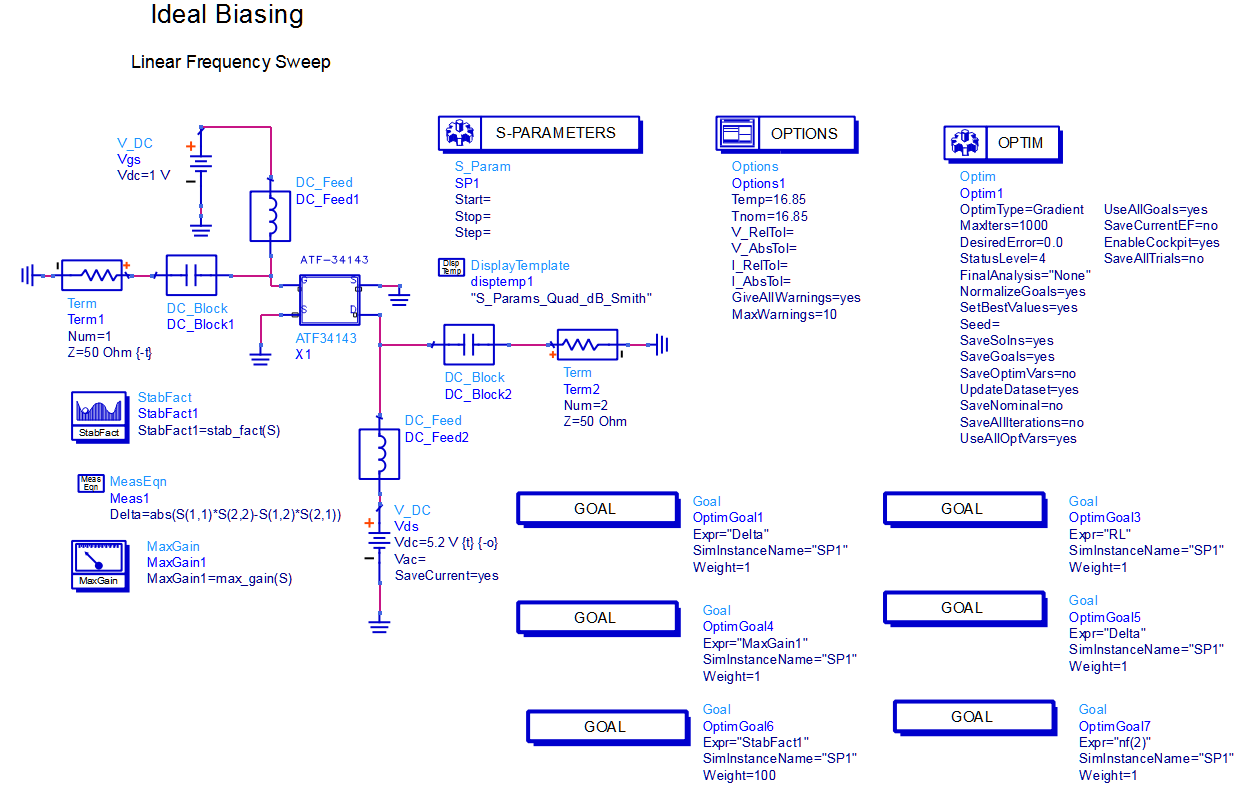
\includegraphics[width=0.8\linewidth]{Images/A2P2IdealSchematic.png}
    \caption{Schematic of the low noise amplifier ideal biasing network}
    \label{fig:A2P2IdealSchematic}
\end{figure}

\begin{figure}[H]
    \centering
    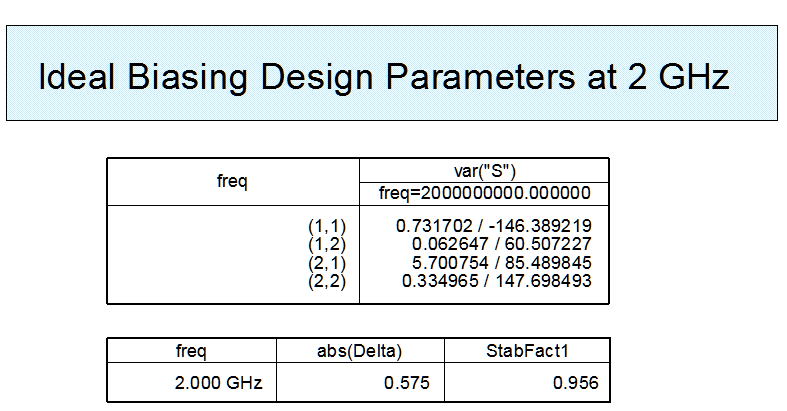
\includegraphics[width=0.8\linewidth]{Images/A2P2IdealBiasingResults.png}
    \caption{Results of the ADS simulation of the low noise amplifier ideal biasing network}
    \label{fig:A2P2IdealBiasingResults}
\end{figure}

\subsection{Physical Biasing}

The schematic and the simulation results of the physical biasing network for the
low noise amplifier are shown in figures \ref{fig:A2P2PhysicalSchematic} and
\ref{fig:A2P2PhysicalResults}, respectively.

Worthy of note: 
\begin{enumerate}
    \item   Figure \ref{fig:A2P2PhysicalResults} indicates stability over the
        entire bandwidth of consideration.
    \item   The return loss is given as $\approx \SI{3.1E-4}{\deci\bel}$.
    \item   The maximum gain at the noise figure selected, $\approx
        \SI{.88}{\deci\bel}$, manages to be quite high at $\SI{2}{\giga\hertz}$:
        $\approx \SI{16.8}{\deci\bel}$.
\end{enumerate}

\begin{figure}[H]
    \centering
    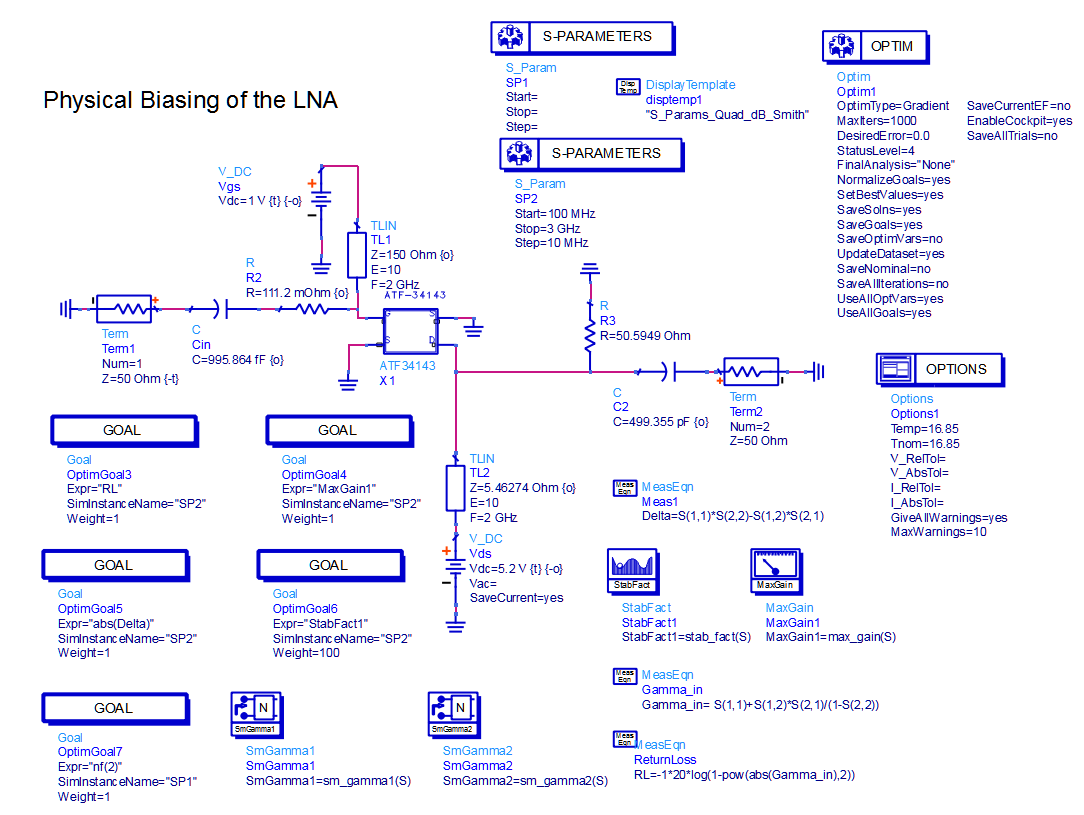
\includegraphics[width=0.8\linewidth]{Images/A2P2PhysicalSchematic.png}
    \caption{Schematic of the physical biasing network for the low noise
    amplifier.}
    \label{fig:A2P2PhysicalSchematic}
\end{figure}

\begin{figure}[H]
    \centering
    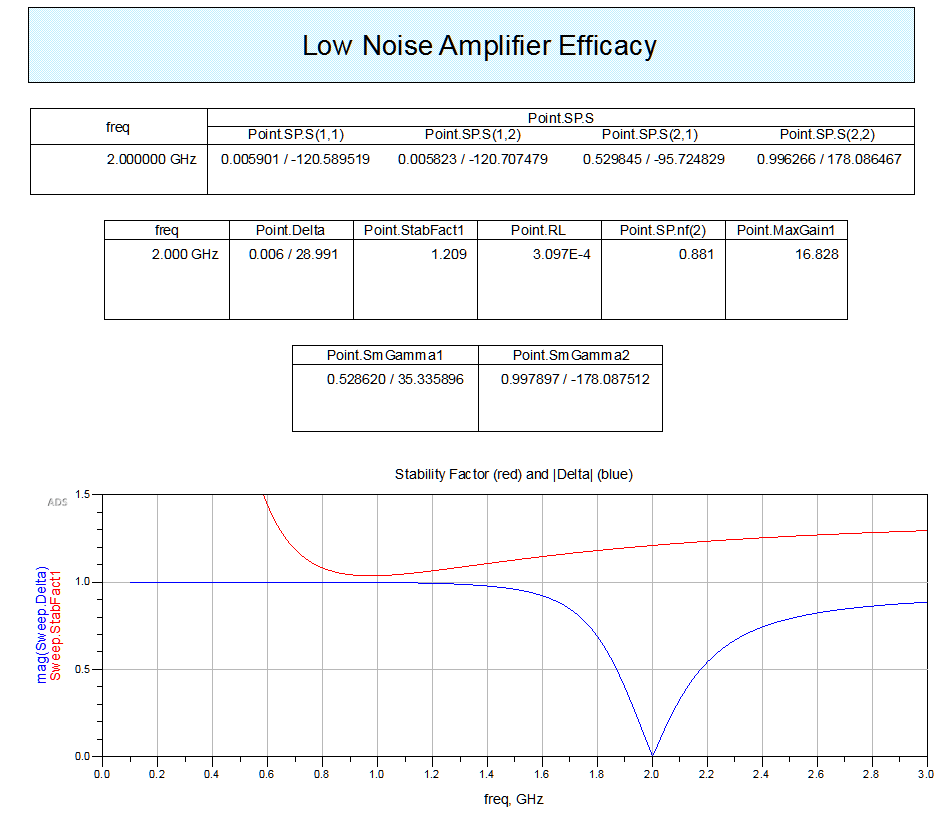
\includegraphics[width=0.8\linewidth]{Images/A2P2PhysicalResults.png}
    \caption{Efficacy of the low-noise amplifier physical biasing network. Note
    the extremely low designed return loss.}
    \label{fig:A2P2PhysicalResults}
\end{figure}

\subsection{Low Noise Amplifier Design}

The full design for the low noise amplifier is shown in figure
\ref{fig:A2P2LNASchematic}. The design efficacy is demonstrated in figures
\ref{fig:A2P2LNADesignFrequencyEfficacy},
\ref{fig:A2P2LNAFrequencySweepStability} and \ref{fig:A2P2LNAFOM}.

\begin{figure}[H]
    \centering
    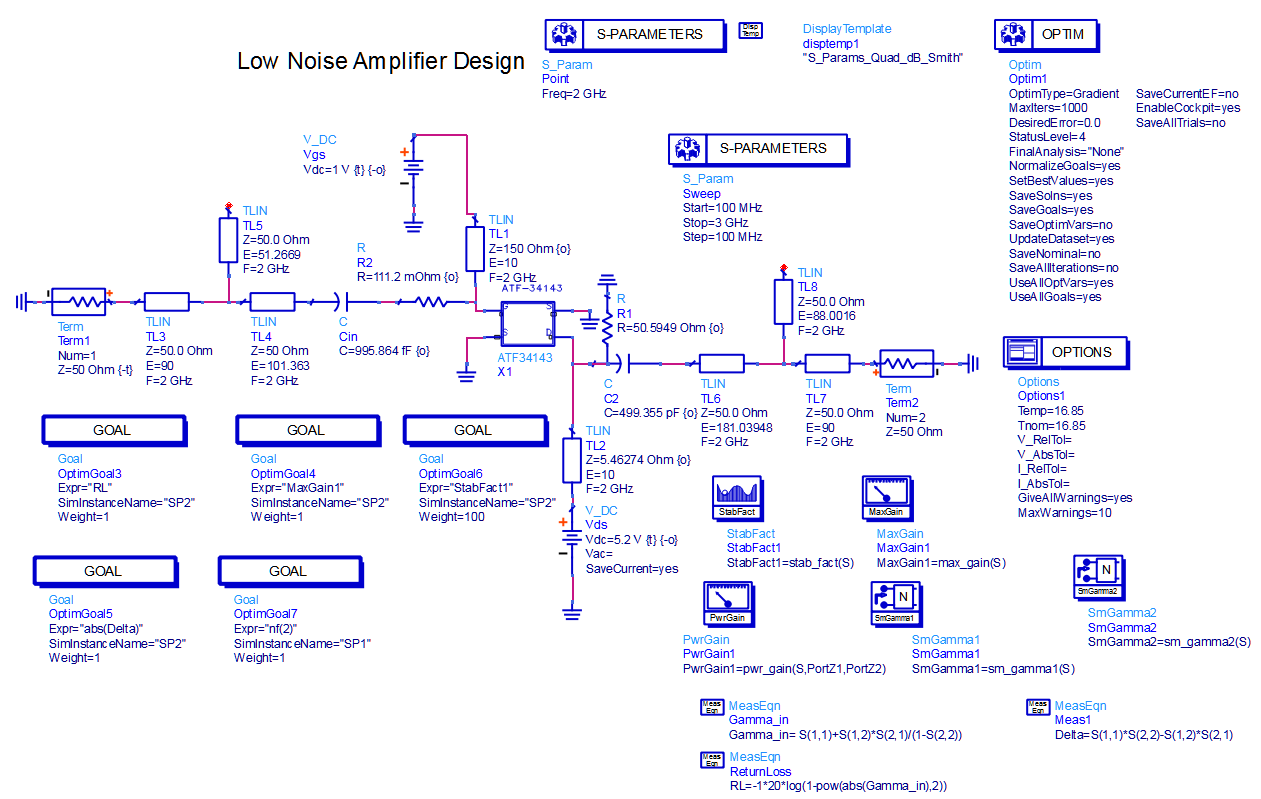
\includegraphics[width=0.8\linewidth]{Images/A2P2LNASchematic.png}
    \caption{Schematic of the LNA design.}
    \label{fig:A2P2LNASchematic}
\end{figure}

\begin{figure}[H]
    \centering
    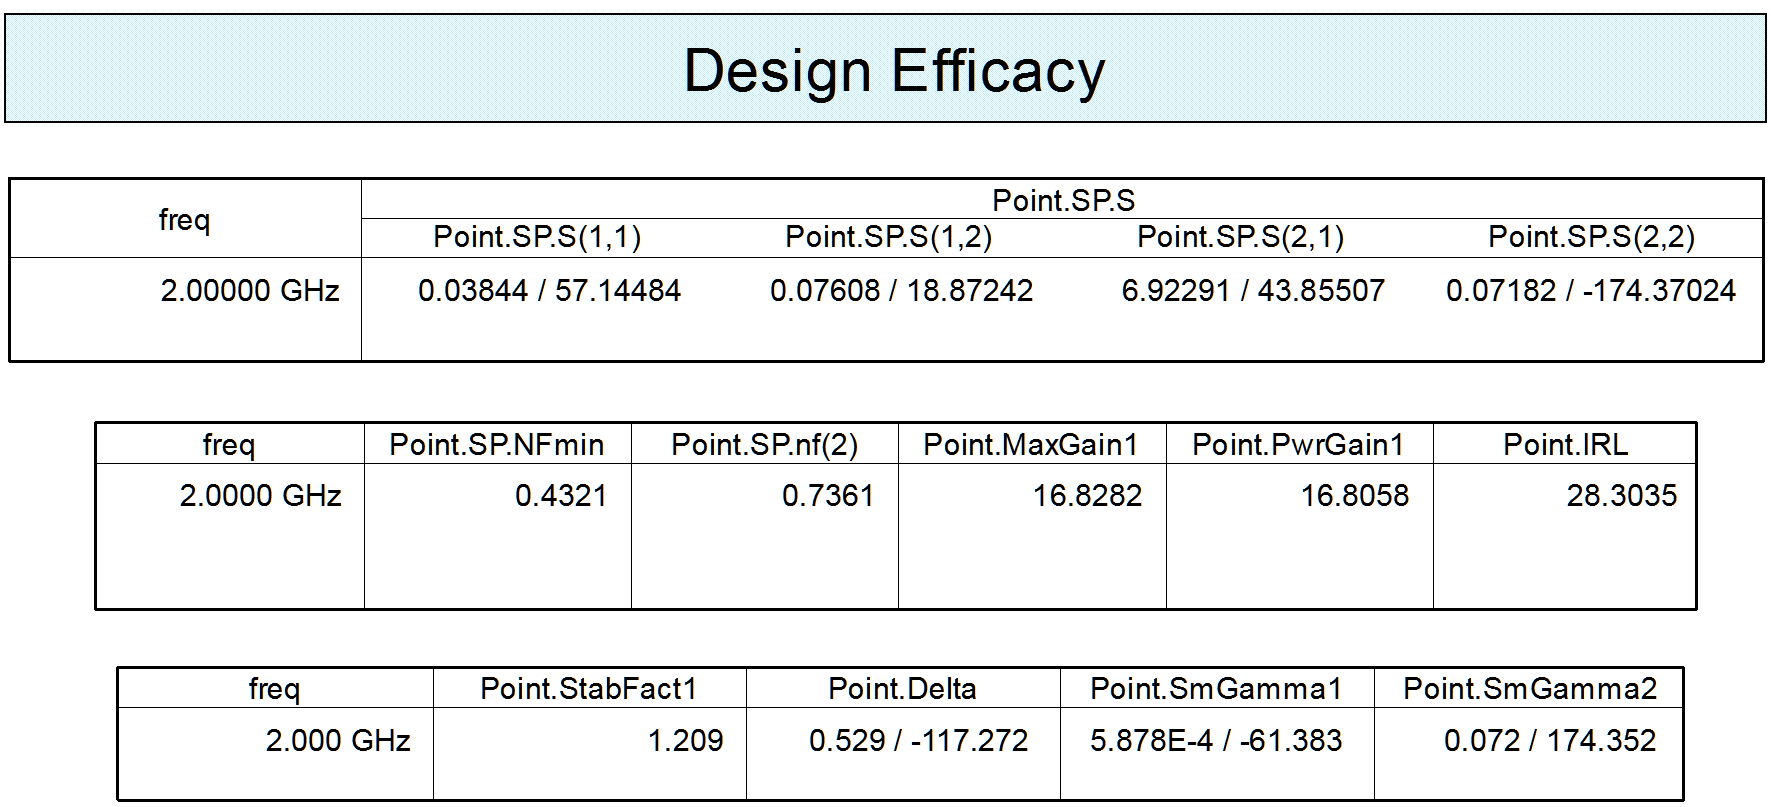
\includegraphics[width=0.8\linewidth]{Images/A2P2LNADesignFrequencyEfficacy.png}
    \caption{LNA efficacy at the design frequency: $\SI{2}{\giga\hertz}$.}
    \label{fig:A2P2LNADesignFrequencyEfficacy}
\end{figure}

\begin{figure}[H]
    \centering
    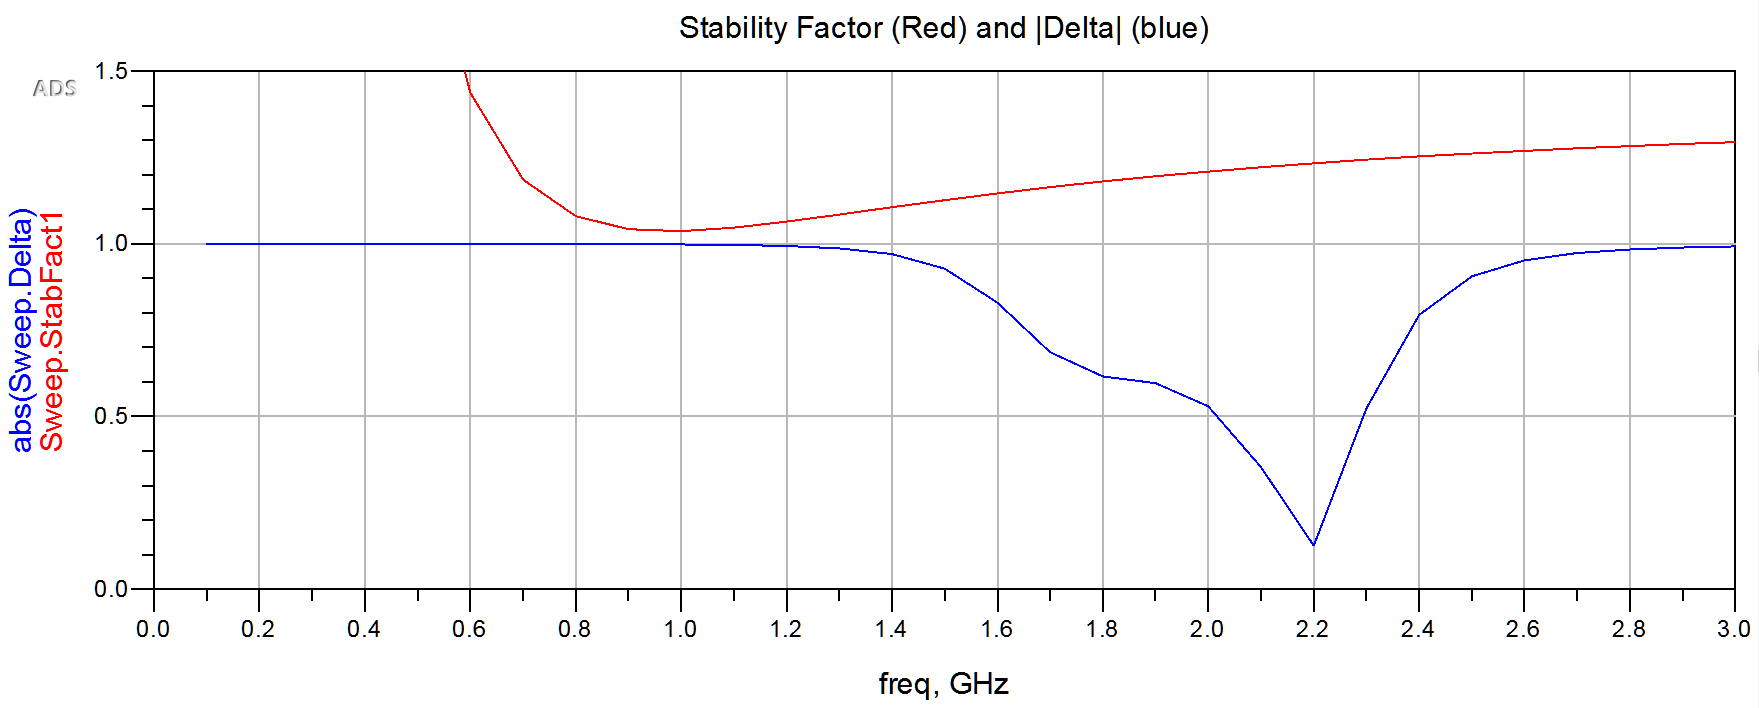
\includegraphics[width=0.8\linewidth]{Images/A2P2LNAFrequencySweepStability.png}
    \caption{LNA stability over the specified bandwidth of the amplifier.}
    \label{fig:A2P2LNAFrequencySweepStability}
\end{figure}

\begin{figure}[H]
    \centering
    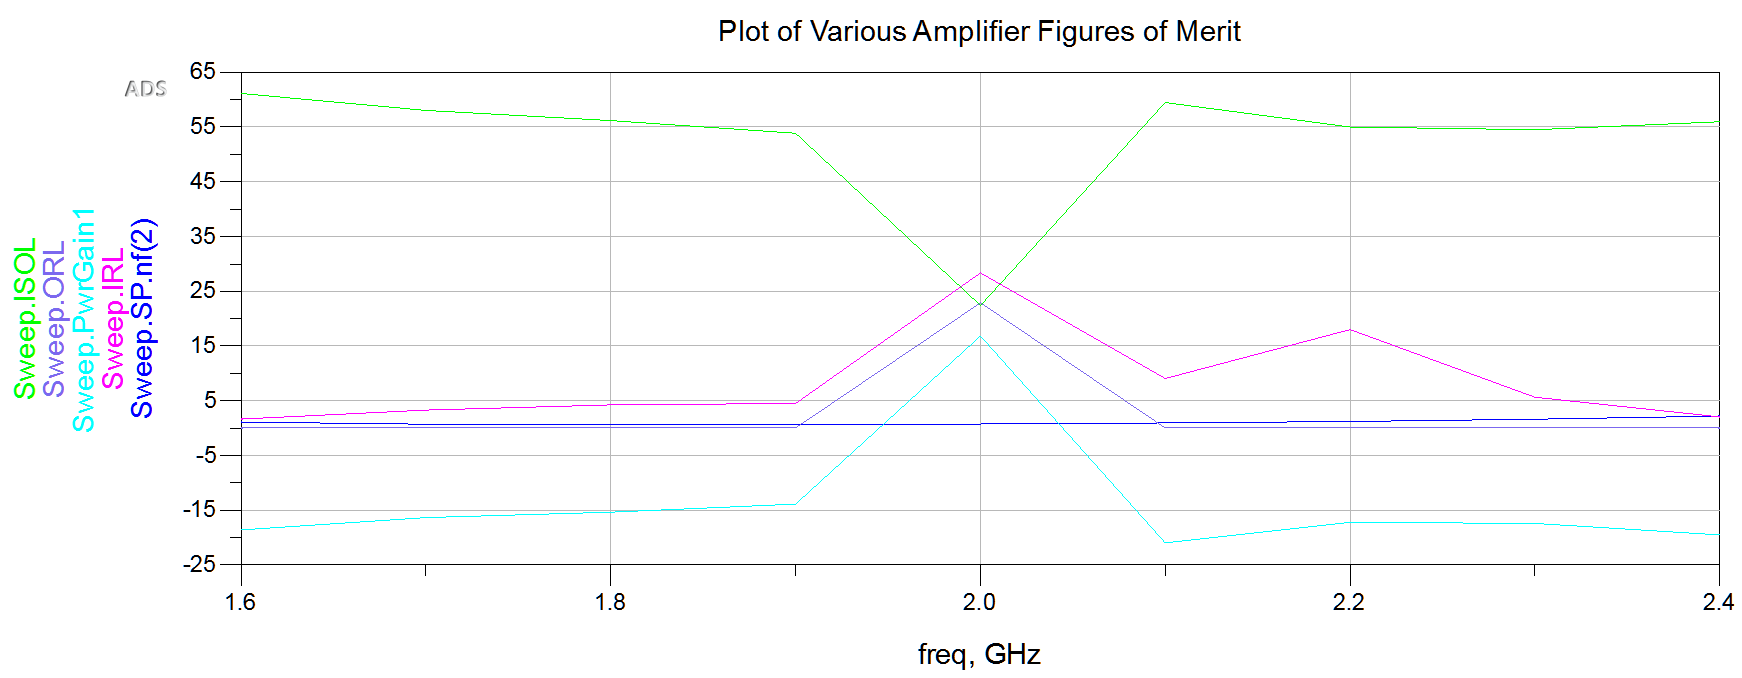
\includegraphics[width=0.8\linewidth]{Images/A2P2LNAFOM.png}
    \caption{Plot of various figures of merit of the amplifier including:
    Isolation (green), output return loss (purple), power gain (teal), input
return loss (pink) and noise figure (blue)}
    \label{fig:A2P2LNAFOM}
\end{figure}

